\begin{frame}\frametitle{Introduction. Standard Model}
\begin{figure}
\label{fig:StandardModel}
\centering 
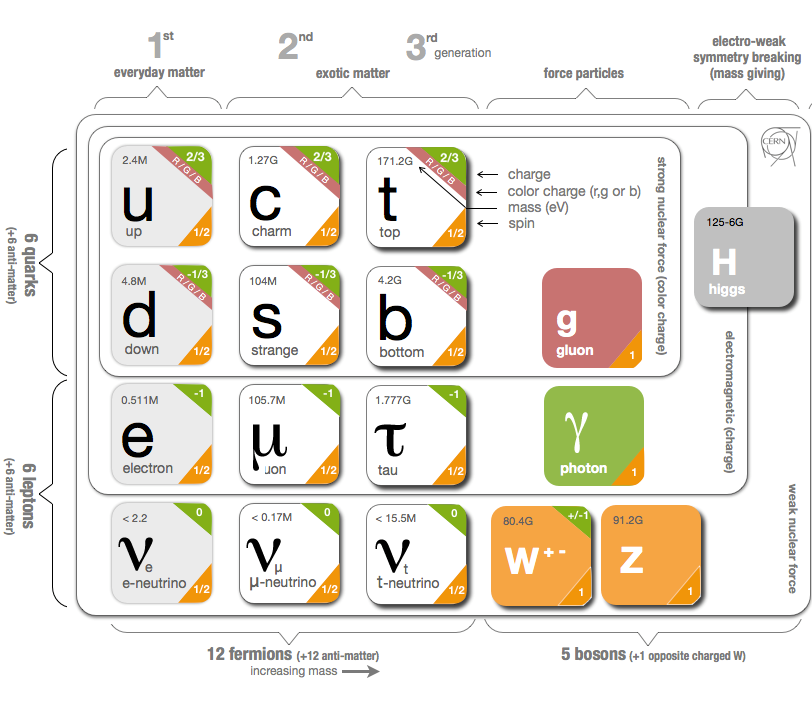
\includegraphics[width=0.75\textwidth, keepaspectratio=true]{figs/StandardModel.png}
\end{figure}
\tiny
All these and only these fundamental particles are discovered at the moment. Source of picture: \cite{ref_fig_StandardModel}
\end{frame}

\begin{frame}\frametitle{Introduction. Neutrino Interactions}
\scriptsize
Feynmann diagrams of neutral current (NC, left), and neutral current (CC, middle and right) neutrino scattering.
\begin{figure}
\label{fig:NuScattering}
\centering
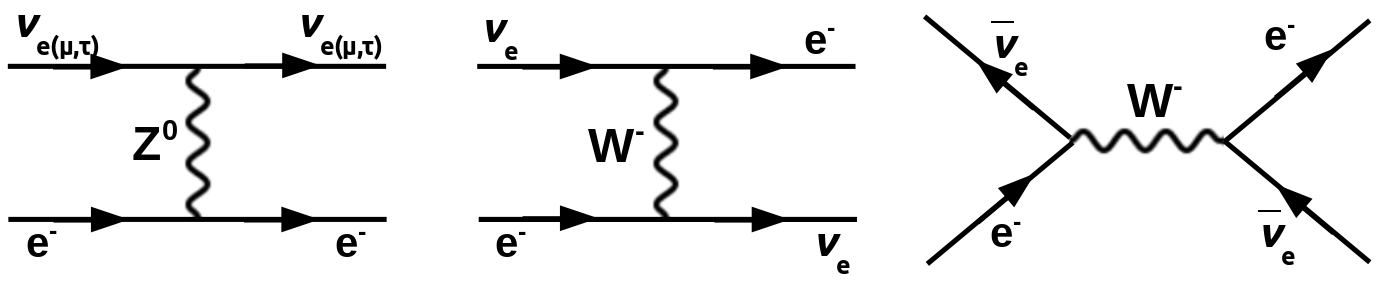
\includegraphics[width=0.90\textwidth, keepaspectratio=true]{figs/neutrinoScattering.png}
\end{figure}
Quoting \cite{ref_Griffiths}, 11.1: "John Bahcall, who was responsible for most of the calculations of solar neutrino abundances, liked to say that 100 billion neutrinos pass through your thumbnail every second; and yet they are so ethereal that you can look forward to only one or two neutrino-induced reaction in your body during your entire lifetime".\\
\end{frame}

\begin{frame}\frametitle{Introduction. Cosmic shower}
\begin{figure}
\caption{Cosmic shower induced by scattering of the incident cosmics proton of an air molecule. Charged and neutron pions are born in the reaction and then they further decay as $\pi^0 \rightarrow \gamma\gamma$, $\pi^+ \rightarrow \mu^+ + \nu_\mu$, $\pi^- \rightarrow \mu^- + \bar{\nu_\mu}$.}
\label{fig:cosmicMuons}
\centering
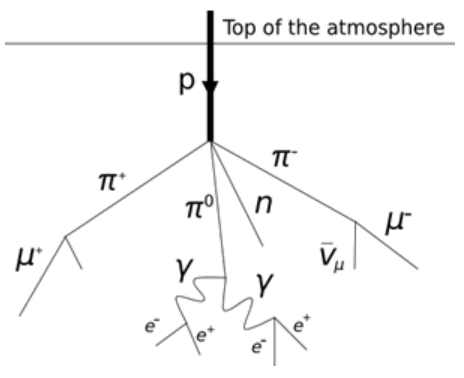
\includegraphics[width=0.60\textwidth, keepaspectratio=true]{figs/cosmicMuons.png}
\end{figure}
\end{frame}

\begin{frame}\frametitle{Introduction. Muon and Neutron Decay}
\scriptsize
\begin{figure}
\caption{Feynmann diagrams of (left) neutron and (right) muon decays. Neutron beta decay \cite{ref_fig_NeutronDecay}(d-quark of transfers to u-quark through the W-boson with emission of electron and antineutrino). Muon decay \cite{ref_fig_MuonDecay}(muon decays to electron, neutrino and antineutrino through W-boson}
\label{fig:MuonAndNeutronDecays}
\centering
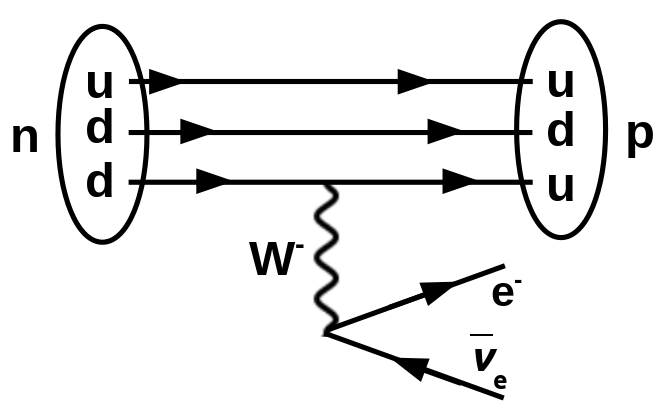
\includegraphics[width=0.35\textwidth, keepaspectratio=true]{figs/NeutronBetaDecay.png}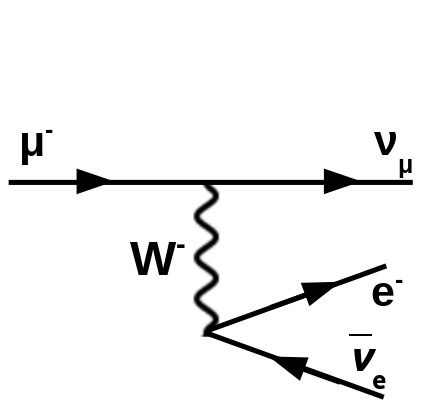
\includegraphics[width=0.35\textwidth, keepaspectratio=true]{figs/MuonDecay.png}
\end{figure}
\end{frame}

\begin{frame}\frametitle{Introduction. Lepton Flavor Number}
\scriptsize
3 flavors of neutrino, one for each generation: $\nu_e$, $\nu_\mu$, $\nu_\tau$. 3 lepton flavor numbers: $L_e$, $L_{\mu}$ and $L_{\tau}$ 

\begin{table}[h]
  \begin{center}
  \caption{ Lepton Flavor Number}
  \begin{tabular}{|c|c|c|c|}
     particles & $L_e$ & $L_{\mu}$ & $L_{\tau}$ \\ \hline
     $e^-,\nu_e$ &  +1  &  0  &  0  \\ \hline 
     $e^+, \bar{\nu_e}$ &  -1  &  0  &  0  \\ \hline 
     $\mu^-,\nu_{\mu}$ &  0  &  +1  &  0  \\ \hline 
     $\mu^+, \bar{\nu_{\mu}}$ &  0  &  -1  &  0  \\ \hline 
     $\tau^-,\nu_{\tau}$ &  0  &  0  &  +1  \\ \hline 
     $\tau^+, \bar{\nu_{\tau}}$ &  0  &  0  &  -1  \\ \hline 
  \end{tabular}
  \label{tab:LeptonFlavorNumber}
  \end{center}
\end{table}
\scriptsize
The lepton flavor numbers are conserved in almost all particle physics processes and the only violation of this law observed by this time is the neutrino oscillations - the ability of neutrino to change flavor. 
\end{frame}
